\chapter{Introduction}
% Main chapter title
\label{Chapter1}
\section{Heparin Sulfate}
Heparin sulfate is a linear oligosaccharide composed mostly of 1,4 linked uronic acid and glucosamine units. It is the most complex member of the glycosaminoglycan family, with a molecular weight approximately between 2,500 and 25,000 Da.  A specific pentasaccharide sequence is necessary to give heparin its anticoagulant ability (Figure \ref{heparin_pentasaccharide}). Consequently, up to 70\%  of a single dose of heparin will remain inactive. Despite the natural biological roles of heparin being poorly understood, it has been used medically as an anticoagulant from as early as 1935.\textsuperscript{\cite{Bromfield2013HeparinApplications}}
\begin{figure} [ht!]
\centering{
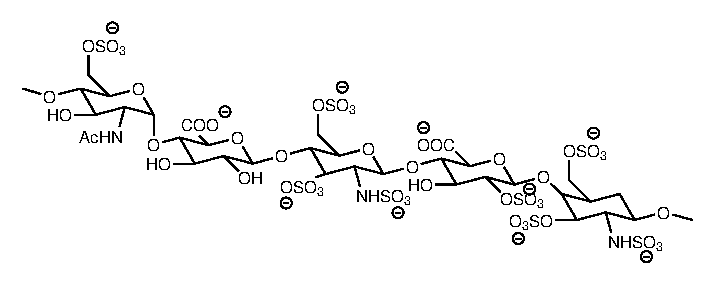
\includegraphics{Figures/heparin_pentasaccharide.eps}}
\caption{Pentasaccharide sequence which gives heparin its characteristic anticoagulant properties. Adapted from \cite{Bromfield2013HeparinApplications,Peterson2009DesignApproach}}
\label{heparin_pentasaccharide}
\end{figure}

There are two separate pathways which control coagulation, as shown in Figure \ref{coagulation_cascade}, “extrinsic” (tissue factor pathway) and “intrinsic” (contact activation pathway), and a pathway which is common to both; unsurprisingly called the common pathway.\textsuperscript{\cite{Sabir2014OralFibrillation}}
\begin{figure} [ht!]
\centering{
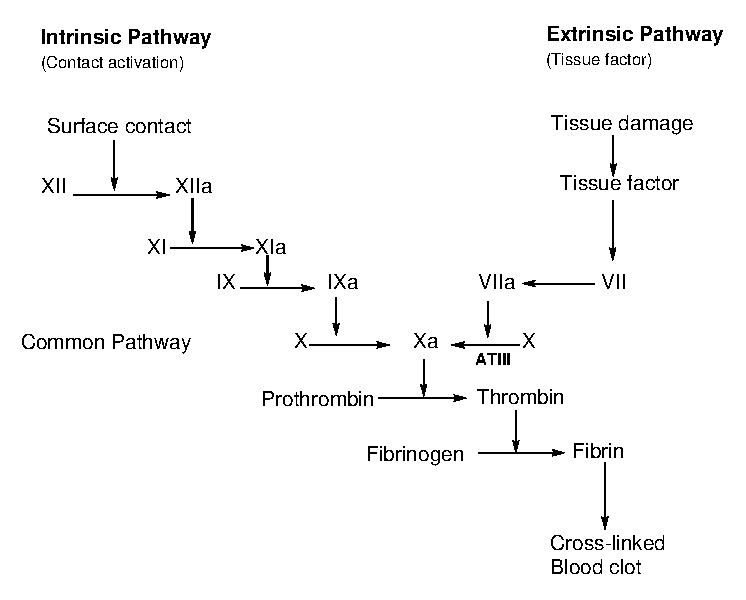
\includegraphics{Figures/coagulation_cascade.eps}}
\caption{The 3 pathways in the coagulation cascade. Roman numerals are used to identify coagulation factors.
Adapted from \cite{Palta2014OverviewSystem.,Peters2013UtilizationTherapeutics,Hirsh2001MechanismHeparin}}
\label{coagulation_cascade}
\end{figure}
\newline
Heparin works by binding to both an enzyme inhibitor known as antithrombin III and if the heparin chain is more than 18 pentasaccharides long, it binds to factor Xa as well.\textsuperscript{\cite{Hirsh2001MechanismHeparin}} This then prevents prothrombin from being converted into thrombin, and interferes with the function of the so-called “common” pathway; a blood clot cannot be formed. 

\subsection{Medical Applications of Heparin Sulfate}
Heparin sulfate finds itself used for a variety of reasons within medicine, most notably as an anticoagulant during major surgery, whether this be during the insertion of a stent to hold cardiac arteries open after a myocardial infarction or during major transplant surgery. In this case, heparin is used to prevent coagulation inside the extracorporeal circuit.\textsuperscript{\cite{BritishMedicalAssociation.2017BNF2017.}} 
\newline
It also finds use as prophylactic treatment for deep vein thrombosis (DVT), even though heparin sulfate cannot break down clots which have already formed, and is used as an additive in the green topped vacutainer vials used in phlebotomy where heparin is used as its lithium salt to prevent coagulation of blood samples.\textsuperscript{\cite{BritishMedicalAssociation.2017BNF2017.}}

\subsection{Issues Associated with Heparin Use}
There are a variety of well-known issues with using heparin as an anticoagulant.
Firstly; as already mentioned, a high proportion of heparin lacks the necessary pentasaccharide sequence that provides its characteristic anticoagulant activity. This causes issues when it is necessary that the total heparin load\footnote{Heparin load - total amount of heparin administered. Includes both the active and inactive parts of heparin.
\newline
Heparin dose - total amount of active heparin. Measured in international units (IU).} is known.   Quantifying heparin levels is typically achieved during surgery \textit{via} an activated clotting time assay. These clotting time based assays are very good at measuring the amount of heparin that is active, but cannot easily determine the heparin load. 
\newline
Secondly, there is an issue with the clotting time based assays themselves. They are slow, and importantly, cannot be performed in situ.\textsuperscript{\cite{Bromfield2013HeparinApplications}} 
\newline
Finally, it is known that not all heparin preparations are the same. Differences arise from the origin of the heparin preparation i.e. bovine vs porcine, in terms of both the structure of the isolated heparin, and its activity.\textsuperscript{\cite{Mulloy2015PharmacologyDrugs}} Bovine sourced heparin can be isolated from both lung and intestinal tissue, whilst porcine sourced heparin is exclusively from intestinal tissue.\textsuperscript{\cite{Tovar2013BovineHaemodialysis.}} Both forms of heparin are often used as if they were indistinguishable in their structure and activity, despite the fact heparin of porcine origin has much higher activity, and hence smaller quantities can be used.  Heparin is provided clinically simply in terms of 'units of activity', with little attention paid to the inactive material. 
\newline
It is important to note that since the 1980's, all licensed heparin products used within the European Union and USA have been of porcine origin, due to the possibility of transmitting variant Creutzfeld-Jakob disease (vCJD) via heparin of bovine origin.\textsuperscript{\cite{Mulloy2015PharmacologyDrugs}}  

\section{Protamine Sulfate}
Protamine sulfate is an arginine-rich cationic peptide of ill-defined structure, often derived from salmon sperm, that is used medically to reverse the anticoagulant behaviour of heparin.\textsuperscript{\cite{Bromfield2013HeparinApplications,Balhorn2007TheProteins}}
Due to issues with the clotting time based assays outlined above, dosing protamine for use as a heparin rescue agent at the end of surgery, is difficult. Dose too much, and the patient will clot too well, potentially be at risk of blood clots forming as well as increasing the risk of developing side effects from protamine sulfate, dose too little and the patient will not clot sufficiently well that healing can begin.
\newline
Finally, the way that protamine itself binds heparin is also problematic, as it makes no distinction between active and inactive parts of heparin, which then leads to larger doses of protamine sulfate being necessary, and hence a greater likelihood of side effects being experienced. Up to 10\% of all those given this rescue agent will have some form of side effect, and those most at risk include those who have had previous treatment with protamine sulfate, insulin-dependent diabetics who take long acting forms containing protamine sulfate, those with a fish allergy and men who are infertile.\textsuperscript{\cite{Bromfield2013HeparinApplications,BritishMedicalAssociation.2017BNF2017.}} 

\subsection{Binding of Protamine Sulfate to Heparin}
The use of protamine sulfate as a rescue agent for heparin is fraught with issues: from the difficulty in dosing, due to the non-selective way it binds to heparin, to the side effect known as heparin rebound first noted by Kolff \textit{et al.} in 1956, where not enough protamine sulfate has been dosed, and as heparin unbinds from plasma proteins, a de-coagulation event and bleeding occurs.\textsuperscript{\cite{Kolff1956DisposableMedicine}} Despite this, protamine sulphate remains the only rescue agent for heparin to gain clinical approval. 
\newline
The binding of protamine sulfate to heparin, which abolishes its anticoagulant ability is based on electrostatic binding. Clearly this opens the possibility of developing systems which can exhibit more selective heparin binding, and potentially only bind to the active polysaccharide sequence, whilst avoiding the side effects associated with the current use of protamine sulfate. 

\section{DNA}
Deoxyribonucleic acid (DNA) contains a varying composition of 4 specific nucleotide bases (guanine, cytosine, adenine and thymine), as well as deoxyribose sugars connected by phosphodiester bonds forming the characteristic sugar-phosphate backbone of DNA.\textsuperscript{\cite{Hamilton2012NaturalBinders}} Hydrogen bonding between these nucleotide bases forms Watson-Crick base pairs (G with C and A with T) and leads to the characteristic double stranded helix known as B-DNA.\textsuperscript{\cite{Voet2011Chapter5}} This B-DNA form has a repeating pattern of wide major grooves, and narrower minor grooves on its surface, in which a variety of molecules can bind (Figure \ref{B-DNA_structure}). 
\begin{figure} [ht!]
\centering{
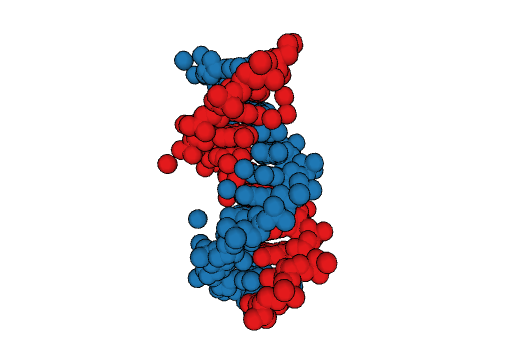
\includegraphics[scale=0.75]{Figures/DNA.png}}
\caption{The repeating pattern of major and minor grooves in B-DNA. From \cite{Nelson1987TheImplications}.}
\label{B-DNA_structure}
\end{figure}
\newline
Heparin sulfate however, is very different to DNA. It is a linear oligosaccharide of varying composition and length, and as such, adopts a very different secondary structure to DNA, instead choosing to form long chains.
Even though there are differences between the roles that DNA and heparin sulfate play within the human body, one being an incredibly important molecule with a well defined, regular structure, which contains all the genetic material necessary for any given living organism; the other being of irregular polymeric structure and used as an anticoagulant, there are similarities between them. Both heparin with its sulfate groups and DNA with phosphate groups are biologically relevant polyanionic molecules.\textsuperscript{\cite{Mulloy2015PharmacologyDrugs}}
\newline
There has been much research into DNA, due to the interest in gene therapy for a variety of congenital disorders not limited to, but including Cystic Fibrosis.
In contrast, there has been comparatively little study of the binding of heparin sulfate to protamine, and even less which attempts to compare and contrast the two.  
\subsection{Binding DNA and Gene Therapy}
%binding to DNA
Small molecules can either interact with DNA in a covalent, or non-covalent fashion. Covalent binding to DNA results in a permanent change in the shape of the DNA binding site, whilst non-covalent interactions are often reversible.\textsuperscript{\cite{Hamilton2012NaturalBinders}} These potentially reversible non-covalent interactions include intercalation between base pairs, electrostatic interactions with the phosphodiester backbone of DNA or interactions with the functional groups of the base pairs in either the major or minor grooves (Table \ref{DNA_binders}).\textsuperscript{\cite{Hamilton2012NaturalBinders,Tuite1997EffectsDichroism}} 

\begin{table}[ht!]
\centering
\caption{A selection of major/minor-groove binders and DNA intercalating agents}
\begin{tabular}{l|l|l}
\textbf{Major-groove binder} &\textbf{Minor-groove binder} &\textbf{Intercalating agent} \\
\hline
Methyl Green& Distamycin A & Ethidium Bromide\\
& & Methylene Blue\\
\end{tabular}
\label{DNA_binders}
\end{table}

It has also been shown by Broggini \textit{et al.}, that the two grooves do not behave independently, as binding distamycin A into the minor-groove leads to interference with the major-groove binding of various regulatory proteins.\textsuperscript{\cite{Broggini1989DistamycinsElements.}}

Gene therapy has the potential to cure cancer, and genetic disorders of both congenital and acquired origin.  For this to be possible, it requires nucleic acids to be transported across the cell membrane by some form of vector, as DNA cannot translocate across cell membranes unaided.\textsuperscript{\cite{Ghosh2008EfficientNanoparticles}} Viral vector methods work well, but there are significant safety concerns with the use of these methods for gene delivery, e.g.  the ability of the vector to revert to wild type, or replication competent virions, the risk of inherent immunogenicity as well as the vector causing an inflammatory response.\textsuperscript{\cite{Ghosh2008EfficientNanoparticles,Kim2016PolycationsApplications}} 

A variety of synthetic vectors have been developed, often based upon polymers, dendrimers or liposomes.  These synthetic vectors avoid some of the issues associated with viral methods, but often suffer from poor loading of genetic material. It is also often difficult to achieve nuclear uptake after cell penetration. It also must be noted that a relatively high molecular weight of the synthetic vector is necessary to lead to effective condensation of DNA, and this high molecular weight often leads to these synthetic systems being cytotoxic.  
There are a variety of cationic polymers which are capable of binding DNA. These include poly-L-lysine (PLL), polyethyleneimine (PEI) as well as PAMAM dendrimers. PLL has been used as a DNA delivery agent for over 20 years due to its relative biocompatibility, and the ease at which it can be degraded by cells.\textsuperscript{\cite{Zauner1998Polylysine-basedDelivery}}  

Cationic lipids have also been used to deliver DNA inside cells. They were first pioneered by Felgner \textit{et al.} in the late 1980's and after further studies, several of these cationic lipid systems are now commercially available.\textsuperscript{\cite{Felgner1987Lipofection:Procedure,Malone1989CationicTransfection}}  
DOTMA (N-[1(2,3-dioleyloxy)propyl]-N,N,N-trimethylammonium chloride) is now sold under the trade name Lipofectin, and DOSPA (2,3-dioleyloxy-N-[2(sperminecarboxido)ethyl]-N,N,-dimethyl-1-propanaminium trifuloroacetate) is sold as Lipofectamine.\textsuperscript{\cite{LipofectinTransfectionReagent-ThermoFisherScientificHttps://www.thermofisher.com/order/catalog/product/18292037,LipofectamineReagent-ThermoFisherScientificHttps://www.thermofisher.com/uk/en/home/brands/product-brand/lipofectamine.html}} 

There are a variety of challenges synthetic vectors must overcome before they can be used as viable transfection methods; these include effective complexation and condensation of the DNA, cellular uptake, and more importantly, endosomal escape as well as nuclear translocation.\textsuperscript{\cite{Ghosh2008EfficientNanoparticles}} Without successful endosomal escape and translocation, the DNA will be transported inside the cell, but not reach the nucleus. 
More recently, CRISPR (Clustered Regularly Interspaced Short Palindromic Repeat)/Cas9 (CRISPR associated gene 9) has been employed as a potential method of genetic delivery. However, once the DNA has been delivered, the CRISPR genes stay behind in the host cell. This has the potential to cause unwanted gene editing - clearly problematic in therapeutic applications, and there is the possibility of immunogenic responses in the host.\textsuperscript{\cite{Mout2017DirectEditing}} 
Various strategies of using CRISPR for genetic editing have been reported in the literature, but they often result in endosomal entrapment of Cas9 and/or single guide RNA (sgRNA).\textsuperscript{\cite{Sun2015Self-AssembledEditing,Zuris2015CationicVivo}}

\subsection{Gene Delivery in Cystic Fibrosis}
Cystic Fibrosis (CF) is a congenital genetic disorder where sufferers receive a faulty copy of the gene which codes for the CFTR (Cystic Fibrosis Transmembrane Conductance Regulator) protein from both parents.
The CFTR gene was not identified until 1989, since then more than 2000 different mutations have been identified.\textsuperscript{\cite{Castellani2017CysticView} } These mutations can be sorted into 6 different classes, based on the type of malfunction within the CFTR protein. 
These mutations differ in the organs that are involved, with lung involvement being most variable. They also differ in the severity of the disorder and the rate of progression. However, these classes cannot be used to predict an individual's outcome with Cystic Fibrosis, as such, these classes are of more use within clinical trials. 

Several theories exist as to how a malfunctioning CFTR protein leads to the symptoms associated with CF.  The most accredited theory states: malfunctioning CFTR protein leads to a lack of water in pericilliary fluid and results in abnormally dense mucus. This mucus is then difficult for the cillia to clear. This faulty protein then causes an increased inflammatory response and decreased activity of natural defense mechanisms, which unsurprisingly facilitates the development of  the symptoms traditionally associated with the disorder, such as repeated lower respiratory tract infections. 
\newline
Research is currently focused on treatments for restoring the function of the CFTR protein, some of which have shown promising results in clinical trials.\textsuperscript{\cite{Castellani2017CysticView}} One way of achieving this would be through intracellular delivery of a correctly functioning copy of the affected gene.  

As genetic therapy advances ever closer towards clinical application, several clinical trials have assessed the potential benefits for a variety of genetic disorders.  A small double-blind study involving 140 CF sufferers was undertaken in 2012 to prove the viability of using inhaled gene-liposome complexes as a potential treatment for some of the respiratory symptoms associated with Cystic Fibrosis.\textsuperscript{\cite{Alton2015RepeatedTrial}} The results show that this certainly isn't a cure for the disorder, but did prevent some decline in lung function. It was noted that further clinical studies of gene delivery vehicles for CF were urgently needed, as this trial did not select participants with a particular type of CFTR mutation, nor could it explain why one group of patients - particularly those with a predicted FEV\textsubscript{1} (forced expiratory volume in 1 second) of <69.2 \% had a greater response than those who were less unwell. 
\section{Multivalent Interactions and Self-Assembly}
In order to bind nanoscale polymeric structures such as heparin or DNA, it is necessary to marshal multiple non-covalent interactions - so called multivalency. As outlined above, systems which can do this may have potential applications in both heparin rescue and/or gene delivery. The cationic polymers and dendrimer systems discussed previously, have been shown to function as potential protamine sulfate mimics, but their toxicity makes medical application unlikely. Also, for even the most simple, first-generation (G1) dendrimers, they often have complex, multi-step syntheses.\textsuperscript{\cite{Rodrigo2011Self-AssemblingBinding}} Due to the difficulty of constructing a covalent array of ligands to bind to a specific target, there has been increasing interest in using self-assembly to organise the multivalent ligands. 

The phenomenon of self assembled multivalency was first reported in 1992 by Whitesides and coworkers in a paper outlining self assembled sugars that bound better to a sugar binding protein than their monovalent counterparts. The polyvalent system is more efficient than the monovalent form – not a surprise considering a central idea of supramolecular chemistry is that polyvalency is superior to monovalency in terms of both efficiency and affinity of binding.\textsuperscript{\cite{Kingery-Wood1992TheGangliosides}} 

\subsection{Self Assembled Multivalency (SAMul)}
Barnard and Smith went on to define self-assembled multivalency in a key review.\textsuperscript{\cite{Barnard2012Self-AssembledBinding}} They defined the phenomenon as relying on small molecules being self assembled into a larger nanostructure, which has the ability to form a multivalent binding array. They noted that this method has a variety of advantages including:
\begin{itemize}
\item spontaneous simple assembly, 
\item well-defined low-molecular-weight building blocks suitable for clinical approval
\item ability to assemble different active components into a single nano-structure
\item simple or triggered disassembly/degradation.\textsuperscript{\cite{Bromfield2013HeparinApplications,Barnard2012Self-AssembledBinding}}
\end{itemize}
The advantages of these SAMul systems come about for a variety of reasons. A carbon chain is often used as the hydrophobe to drive self-assembly. The spontaneous assembly arises from a fine balance between hydrophobic and hydrophilic components of the molecule.   
\newline 
Triggered bond cleavage of these systems is possible by inserting, for example, an ester group between the hydrophobic tail and hydrophilic binding group. Ester groups are well known to degrade under biological conditions. When the ester undergoes hydrolysis, the molecule breaks apart and self assembly of the system is no longer possible. Once the molecule loses the ability to self assemble, its binding ability is then "switched off". 
%insert cartoon of self-assembly here
\newline
Degradation and disassembly then also limits the biopersistance of the molecule and helps with issues of toxicity that can be present with polymeric multivalent binding systems.\textsuperscript{\cite{Rodrigo2011Self-AssemblingBinding, Barnard2012Self-AssembledBinding}}

\newpage
\section{Potential Protamine Sulfate Mimics}
A variety of different research groups have attempted to synthesise a biologically compatible protamine sulfate mimic, and several alternate approaches have been used. These include:
\begin{itemize}
\item  cationic polymers and dendrimers
\item protein based heparin binders
\item small molecules
\item Self-Assembled Multivalency (SAMul)
\end{itemize}
\subsection{Cationic Polymers and Dendrimers}
A popular approach for developing synthetic protamine sulfate mimics is to base the structure on a large cationic compound which binds heparin via multiple electrostatic interactions. Both multivalent cationic polymers and dendrimers (branched macromolecules of regular, well defined structure) have been used, and can achieve high binding affinity to heparin. However, cationic polymers tend to be biopersistant and hence toxic – this can be a problem.\textsuperscript{\cite{Rodrigo2011Self-AssemblingBinding, Barnard2012Self-AssembledBinding}}
It has been shown by Fr\'{e}chet \textit{et al.} that neutral, low generation dendrimers are water soluble, and likely to be more suitable for medical applications.\textsuperscript{\cite{PadillaDeJesus2002PolyesterEvaluation}}

\begin{figure} [ht!]
\centering

\includegraphics[scale=1.0]{Figures/PAH_structure.eps}
\caption{Structure of Poly(allylamine hydrochloride)}
\label{PAH_structure}
\end{figure}

Functionalised poly(allylamine hydrochloride) (PAH) derivatives have  been trialled as potential protamine sulfate mimics. Naturally derived polymers have issues with batch-to-batch variation, and hence, it was argued that a synthetic polymer is more appealing.\textsuperscript{\cite{Kaminski2014NewReversal}} Kami\'{n}ski \textit{et al.} chose to use a poly(allylamine hydrochloride) backbone as it already finds a variety of uses within medicine and therefore, it was possible that a functionalised derivative of this would also be biologically compatible. The scaffold was then functionalised with arginine groups, to enable it to bind heparin in the same manner as protamine sulfate.  Azure A displacement assays showed that the dose of this arginine-functionalised PAH derivative required to neutralise a 1 mg dose of heparin was less than half that of protamine sulfate (0.46 mg).\textsuperscript{\cite{Kaminski2014NewReversal}} Cytotoxicity studies were also performed and showed that the functionalised PAH derivative was less cytotoxic than the PAH scaffold alone. 

\begin{figure} [ht!]
\centering
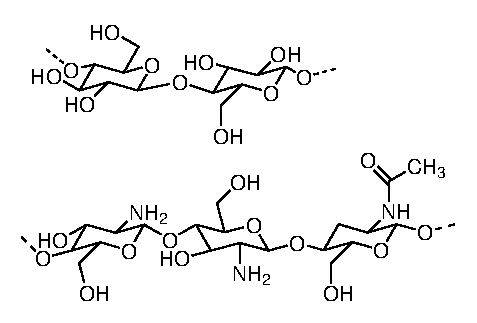
\includegraphics[scale=1.0]{Figures/dextran+chitosan_structure.eps}
\caption{Top: structure of dextran. \newline
Bottom: structure of chitosan.}
\label{dextran+chitosan_structure}
\end{figure}
Kami\'{n}ski \textit{et al.} also developed cationic derivatives of chitosan and dextran. \textit{ In vitro} and \textit{in vivo} testing of these compounds was positive.\textsuperscript{\cite{Kaminski2014NewReversal}}  Notably, no immunogenic response was shown, and they act as effective heparin antidotes. However, in rat models, it has been shown that these compounds are not completely free of side effects. The chitosan derivatives interact with erythrocytes while dextran derivatives cause hypotension - like protamine sulfate.\textsuperscript{\cite{Kaminski2014NewReversal}} 

Dex40-GTMAC3 is a functionalised dextran derivative with an average molecular weight of 40 kDa, and functionalised with glycidyltrimethylammonium chloride (GTMAC) at a ratio of 0.65 GTMAC groups per glucose unit.\textsuperscript{\cite{Sokolowska2016TheHeparin}} Recently published work shows that these functionalised dextrans are non-toxic, biodegradeable and function well as protamine sulfate mimics.\textsuperscript{\cite{Kalaska2015NonclinicalHeparin}} Toxicology studies on rats have shown that there is rapid renal clearance of the drug, with plasma concentration falling to less than half of that administered after 10 minutes, and little in terms of tissue accumulation.\textsuperscript{\cite{Kalaska2015NonclinicalHeparin}}  Therefore, this dextran derivative is much better tolerated than protamine sulfate. However, the researchers are aware much more testing needs to be done before this functionalised dextran derivative can enter clinical trials. 

\subsection{Proteins, Peptides and Peptoids}
Ford, Hamza and Rabenstein used N-substituted glycine peptoids, generated systematically by solid-phase synthesis.\textsuperscript{\cite{Ford2013DesignPeptoids}} The use of substiuted peptoids (Figure \ref{peptide_vs_peptoid}) rather than peptides, leads to several advantages, particularly when considering the use of these molecules as potential drug candidates. Peptoids are resistant to proteases unlike peptides and are better able to pass through biological membranes. Most importantly as potential protamine sulfate mimics, they do not trigger an immunogenic response. 
\begin{figure} [ht!]
\centering
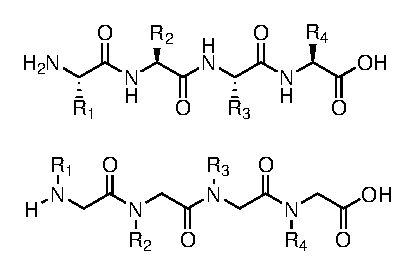
\includegraphics{Figures/peptide_vs_peptoid.eps}
\caption{Generic tetrapeptide (top) and generic tetrapeptoid (bottom). Adapted from \cite{Ford2013DesignPeptoids}}
\label{peptide_vs_peptoid}
\end{figure}

It was discovered by Carson and coworkers that there is a naturally occurring heparin interacting protein (HIP) present in human uterine epithelial cells, and subsequently the heparin binding domain of this protein was sequenced.\textsuperscript{\cite{Rohde1996CellLines.,Liu1996CDNALines.}} 
In 2006, two synthetic analogues (Figure \ref{HIPAP_structure}) of this heparin interacting protein were synthesised by Wang and Rabenstein.\textsuperscript{\cite{Wang2006Interactionsup/sup}}

\begin{figure} [h!]
\centering
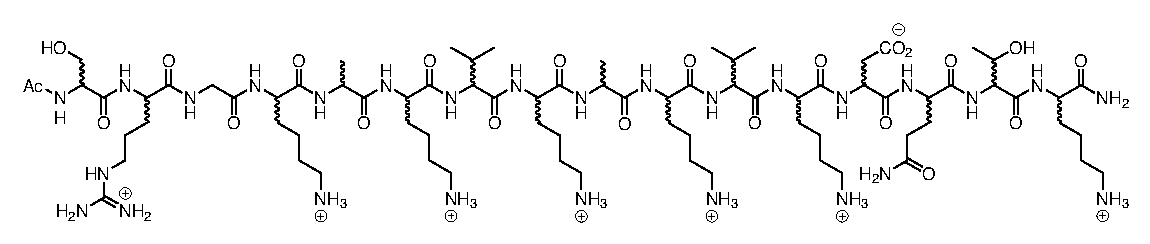
\includegraphics[scale=0.85]{Figures/HIPAP_structure.eps}
\caption{Structure of HIPAP. Adapted from \cite{Wang2006Interactionsup/sup}.}
\label{HIPAP_structure}
\end{figure}

These heparin interacting protein analogue peptides (HIPAP) differed from each other only in the chirality of the amino acids that were used. One used purely the endogenous L-form, and the other, purely D-forms of the amino acids.  It was noted that both L-HIPAP and D-HIPAP are capable of binding heparin, neutralising its anticoagulant activity, and that they are equally effective. It was also shown that the spatial arrangement of the six lysines and the one arginine residue play an important role in the heparin binding ability, as a scrambled version of this peptide did not effectively bind heparin. These observations suggest that charge density and spacial organisation of charge, not chirality, are the most dominant forces in these heparin-binding systems. 

\subsection{Small Molecule-Based Heparin Binders}
There have been several small molecule based heparin binders reported in the literature. Key examples include delparantag, ciparantag and functionalised calix[8]arenes.\textsuperscript{\cite{Bromfield2013HeparinApplications}} 
\begin{figure} [h!]
\centering
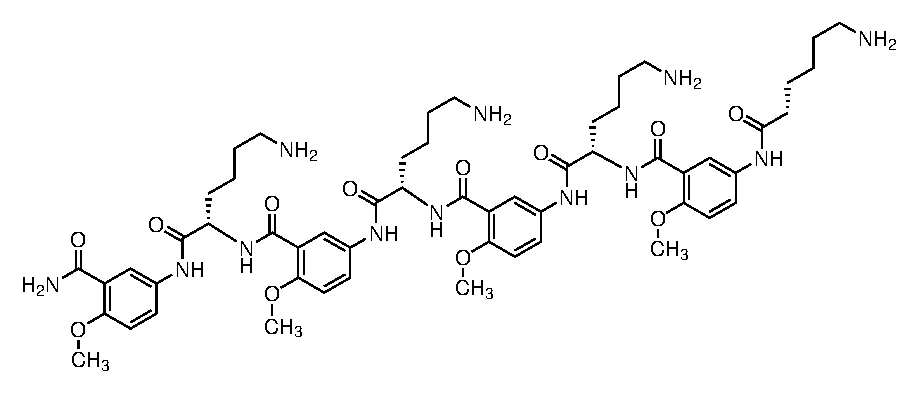
\includegraphics[scale=0.85]{Figures/delparantag_structure.eps}
\caption{Structure of Delparantag. Adapted from \cite{Mahan2014AAgents}.}
\label{delparantag_structure}
\end{figure}

Delparantag (PMX-60056) is a novel salicylamide-derived small molecule with a molecular weight of 1,126 Da.\textsuperscript{\cite{Mahan2014AAgents}} It was designed to interact with the pentasaccharide sequence and prevent the interaction with antithrombin III. It underwent several phase IB/II trials and showed promising results, notably being one of the few potential protamine sulfate mimics capable of full reversal of the effects of both unfractionated heparin (UFH) and  low molecular weight heparins (LMWH).\textsuperscript{\cite{Mahan2014AAgents,Kuziej2010InDerivative}}
However, the trial was halted and then terminated in May 2012 due to participants developing hypotension on administration of Delparantag.\textsuperscript{\cite{ReversalClinicalTrials.gov}} No further trials are currently in progress.

\begin{figure} [h!]
\centering
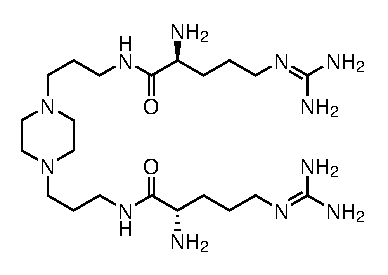
\includegraphics[scale=0.85]{Figures/ciraparantag_structure.eps}
\caption{Structure of ciraparantag.}
\label{ciraparantag_structure}
\end{figure}

Ciraparantag (PER977) (Figure \ref{ciraparantag_structure}) is another synthetic, water soluble cationic molecule designed specifically to bind to both LMWH and UFH by non-covalent hydrogen bonding and electrostatic interactions.\textsuperscript{\cite{Ansell2014UseEdoxaban}} It is currently undergoing phase II trials, and if shown to be both safe and effective, it could become the first broad-spectrum rescue agent for novel oral anticoagulants (NOAC). 

It has already been shown that ciraparantag restores baseline haemostasis within 30 minutes of administration, is well tolerated by patients, and does not interact with several other drugs.\textsuperscript{\cite{Ansell2014UseEdoxaban,Ansell2016CiraparantagHeparin}} The interaction of ciraparantag was assessed with the anticonvulsives lamotrigine and carbamazepine (the latter also finding itself used as a mood stabiliser in bipolar disorder), and several cardiac medications including the antiplatelet drug clopidogrel, which is useful in the case of patients undergoing polypharmacotherapy.\textsuperscript{\cite{BritishMedicalAssociation.2017BNF2017.,Laulicht2013AntidoteEdoxaban}}

\begin{figure} [h!]
\centering
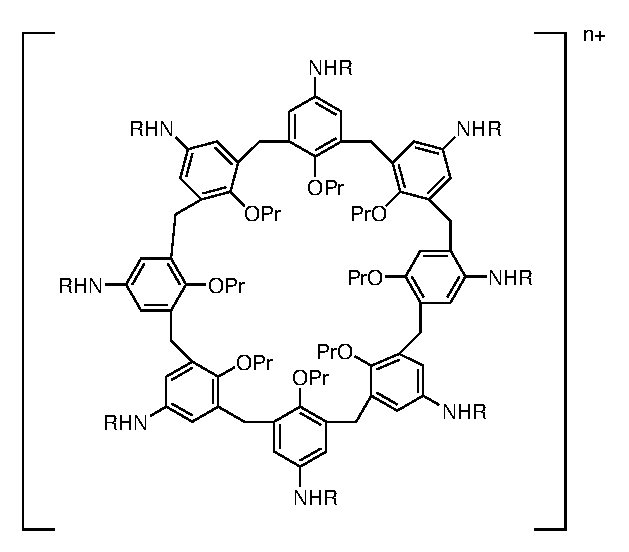
\includegraphics[scale=0.75]{Figures/calix_8_arene.eps}
\caption{Structure of the functionalised calix[8]arene synthesised by Cunsolo \textit{et al.} Adapted from \cite{Mecca2006PolycationicHeparin}.}
\label{calix[8]arene_scaffold}
\end{figure}

Functionalised calix[8]arenes were reported by Cunsolo \textit{et al.} in 2006 as potential protamine sulfate mimics. The calix[8]arene scaffold (Figure \ref{calix[8]arene_scaffold}) was chosen due to its conformational adaptability. Two different functionalised calix[8]arene scaffolds were synthesised in order to probe the effect of charge density on the binding affinity towards heparin. It was also hypothesised by the researchers that the flexibility of both the calix[8]arene and heparin would improve binding affinity. 
On comparison of the results for binding heparin to protamine sulfate, this was shown to be true, as the rigid structure of protamine negatively affected the rate of complexation.\textsuperscript{\cite{Mecca2006PolycationicHeparin}} 
\newpage
It was also shown that the rate of complexation is affected more strongly by the adaptability and flexibility of the host:guest complex, than by simple charge density. 

\subsection{Self-Assembled Multivalency (SAMul)}
Self-assembled multivalency (SAMul) has also been employed as a method by which novel protamine sulfate mimics could be produced. This approach is very different to that used by Ford and Rabenstein, and has a variety of advantages which have already been outlined above. Particularly useful is the ability to combine several components into a single structure, and the possibility for simple or triggered disassembly. 

The use of SAMul in the development of nanoscale self-assembling heparin binders was first reported in the literature by Campo-Rodrigo, Barnard \textit{et al.} in 2011.\textsuperscript{\cite{Rodrigo2011Self-AssemblingBinding}} This paper showed that a self-assembling dendron (Figure \ref{C22-G1_structure}) could be used to bind heparin when functionalised with amines, that are protonated at physiological pH, and a hydrophobic group is necessary to drive the self-assembly. This implies that at least part of binding the self-assembled nanoscale interface to heparin has an electrostatic component. However, it was also noticed by the researchers that the synthesis of this system was certainly not facile, and that significant further work was necessary to probe the ability of this dendron to disassemble and degrade, as it was already known that dendrimers are biopersistent and can be toxic.
\begin{figure} [h!]
\centering
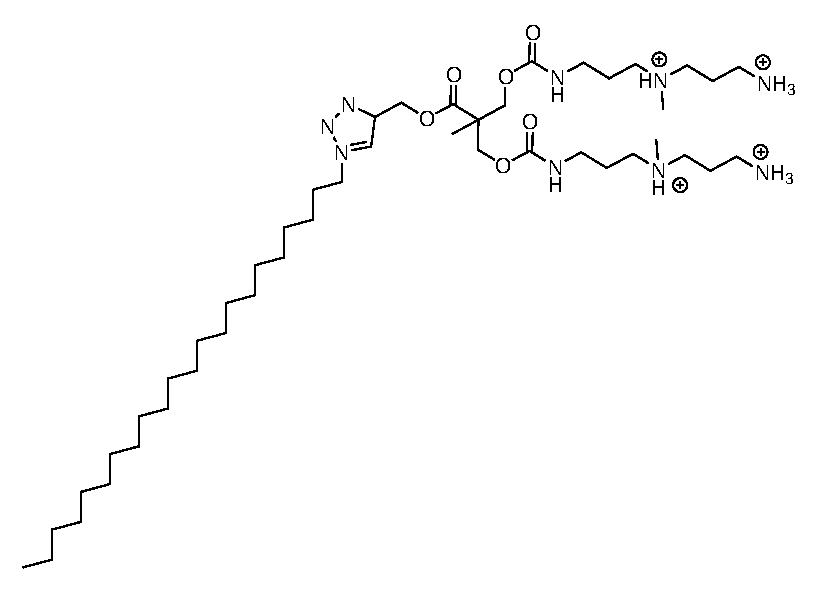
\includegraphics[scale=0.75]{Figures/G1_structure.eps}
\caption{Structure of the C22-G1 self-assembling dendron synthesised by Campo-Rodrigo \textit{et al.} Adapted from \cite{Rodrigo2011Self-AssemblingBinding}.}
\label{C22-G1_structure}
\end{figure}

Further work was carried out on this system by Bromfield \textit{et al.} to probe whether this self-assembling "pseudo-dendrimer" was still as effective at binding heparin in biologically competitive media.\textsuperscript{\cite{Bromfield2014NanoscaleMedia}} The binding assays in the Campo-Rodrigo paper were only performed in phosphate buffered saline (PBS), which bears little resemblance to human serum in terms of the electrolytes that it contains. Therefore, the assays to assess heparin binding were performed in a solution of 150 mM NaCl and 10 mM Tris-HCl. It was shown that C22-G1 still self-assembles in solution, and the increased salt concentration increases the size of the self-assembled micelle. This is unsurprising as increasing the ionic strength of a solution is known to increase both the screening of surface charge and the impact of the hydrophobic effect.\textsuperscript{\cite{Bromfield2014NanoscaleMedia}} This then leads to a greater number of individual molecules being included in the self-assembled micelle, hence increasing its diameter.

Bromfield then went on to assess the self-assembly of C22-G1 in human serum. Human serum contains all the electrolytes and blood components found within human blood, with the exception of those involved in blood clotting.\textsuperscript{\cite{Bromfield2014NanoscaleMedia}} It was hoped that if this system could still function in human serum, and be a more effective heparin binder than the currently utilised protamine sulfate, then medical application of these self-assembling pseudo-dendrimers could become reality.  Unfortunately, the results showed that C22-G1 becomes less effective as a heparin sulfate binder in human serum, with its CE\textsubscript{50} value rising from 0.28 to 0.96. However, the compound was demonstrated in some clotting assays to still function optimally in human plasma.\textsuperscript{\cite{Bromfield2014NanoscaleMedia}} 

The effect of flexibility on binding self-assembling nanoscale interfaces to heparin and/or DNA, was then studied. Fechner, Albanyan \textit{et al.} modified only the binding group and kept the hydrophobic component of their systems the same.\textsuperscript{\cite{Fechner2016ElectrostaticBinding}} This work showed that certain binding groups had a greater binding affinity to heparin/ DNA than others (Figure \ref{SPM_vs_SPD}). 
\begin{figure} [ht!]
\centering
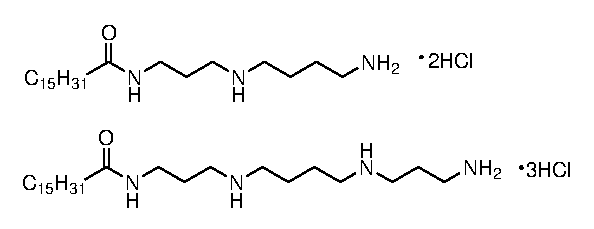
\includegraphics[scale=0.9]{Figures/SPM_vs_SPD.eps}
\caption{The differences in structure between spermidine (above) and spermine (below). From \cite{Fechner2016ElectrostaticBinding}.}
\label{SPM_vs_SPD}
\end{figure}

The self-assembling interfaces with spermidine ligands had a greater affinity for heparin, whilst those with spermine ligands had greater affinity for DNA. It was also noted that DNA appears to be a “shape-persistent” polyanion, which will attempt to organise the SAMul assembly that it is presented with. In contrast, Heparin is a “adaptive” polyanion, which changes itself in response to the SAMul binding surface.\textsuperscript{\cite{Fechner2016ElectrostaticBinding}} These results also strongly agree with the arguments made by Cunsolo \textit{et al.} that the flexibility of heparin also plays a key role in binding.\textsuperscript{\cite{Mecca2006PolycationicHeparin}}

Over the past 6 years, the structure of these self-assembling nanoscale heparin binders has been repeatedly modified, and is now very different to the structure originally used by Campo-Rodrigo and Barnard.\textsuperscript{\cite{Rodrigo2011Self-AssemblingBinding}} It is no longer a first generation dendron, but a small, discrete molecule capable of self assembly. These molecules now consist of a hydrophobic carbon chain, used to encourage the molecule to self-assemble in aqueous media, and a binding group displayed on the outside of the self-assembled micelle, which is positively charged at physiological pH. 

More recently, work has been published exploring the effect of modifying the hydrophobic carbon chain on binding of these nanoscale systems to both heparin and DNA. Vieira, Liljestr\"om \textit{et al.} used C14-DAPMA, C16-DAPMA and C18-DAPMA to assess the effect of changing hydrophobic chain length on binding to heparin sulfate.\textsuperscript{\cite{Vieira2017EmergenceHeparin}}  It was noted that altering hydrophobic chain length had an effect on the solubility of these nanostructures, as C18-DAPMA was poorly soluble in PBS buffer.  The measured \textzeta - potentials also highlighted the effect changing the length of the carbon chain has on the ability of the molecule to self-assemble. The greater the \textzeta-potential, the greater the driving force required for self assembly, and this is seen to increase with increasing chain length.  Albanyan, Laurini \textit{et al.} also modified the hydrophobic chain by changing the number of double bonds along its length.\textsuperscript{\cite{Albanyan2017Self-AssembledLigands}} The self-assembly of these structures was quantified using Nile Red assays, and it was shown that increasing numbers of double bonds increased both critical micelle concentration, as well as the diameter of the self-assembled micelles. Surprisingly, results also showed that altering the number of double bonds in the carbon chain alters the selectivity of these systems towards both DNA and heparin. C18-1 shows a strong preference towards heparin binding relative to that for DNA, whilst the results are the reverse for C18-3. This is believed to occur because of the degree of preorganisation imparted into the molecule by increasing numbers of cis double bonds and the "shape-persistant" behaviour of DNA. 

\begin{figure} [ht!]
\centering
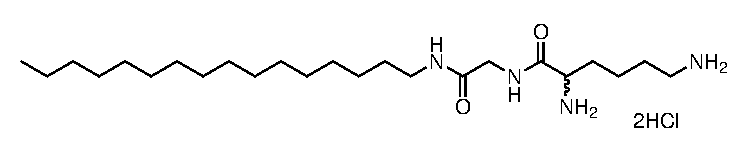
\includegraphics{Figures/C16-Gly-Lys.eps}
\caption{The self-assembling nanoscale binder developed by Chan et al. From \cite{Chan2016ChiralBinding}.}
\label{C16-Gly-Lys}
\end{figure}

Finally, it has been noted that these newer self-assembling nanoscale binders can also display chiral selectivity (Figure \ref{C16-Gly-Lys}).  It is known that a SAMul binder composed of only palmitic acid and a L/D-lysine binding group will bind to heparin and DNA, but display no chiral preference.\textsuperscript{\cite{Chan2016ChiralBinding}} On insertion of an amino acid spacer group, in this case glycine, chiral selectivity was "switched on".  This chiral selectivity is useful as it enables us to tune the selectivity of the SAMul interface towards a particular biological polyanion. Binding assays show that C\textsubscript{16}-Gly-D-Lys has a much improved affinity for DNA compared to its analogous L-lysine containing counterpart, and it was suggested that the insertion of the glycine spacer group enables the molecule to "better express its chirality", as the insertion of the glycine spacer group modifies both the shape and polarity.\textsuperscript{\cite{Chan2016ChiralBinding}} It was also suggested that the addition of a glycine spacer leads to additional hydrogen bonding sites and potentially modifies the binding between the SAMul system and binding partner.  As a consequence, it is believed that this chiral selectivity may remain, if the spacer group is changed from glycine to another chiral amino acid. 

Using self-assembly to create systems capable of inhibiting the function of heparin sulfate has not only been explored by Smith and coworkers. In 2014, DeGrado \textit{et al.} published a paper in which the phenomenon of self-assembly was applied to create heparin-binding foldamers.\textsuperscript{\cite{Montalvo2014DeInteractions}} Foldamers are non-biological sequence specific polymers of a defined length, which also possess well defined secondary and tertiary structures. They are often used to assess the folding and function of various biomacromolecules and have been used more recently to inhibit protein-protein interactions. The foldamers used by DeGrado \textit{et al.} were based on a repeating pattern of lysine and 5-amino-2-methoxy-benzoic acid (Sal) units (Figure \ref{Lys-Sal_foldamer}).

\begin{figure} [ht!]
\centering
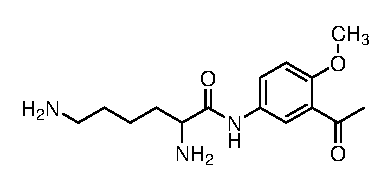
\includegraphics{Figures/Lys-Sal_foldamer.eps}
\caption{Repeating Lys-Sal unit in the heparin-binding foldamers used by DeGrado \textit{et al.} From \cite{Montalvo2014DeInteractions}.}
\label{Lys-Sal_foldamer}
\end{figure}

The results showed that the binding affinity of these Lys-Sal foldamers did not depend on the chirality of the lysine side chains, and that like the nanoscale SAMul systems developed by Chan \textit{et al.}, self-assembly of the foldamer is necessary before heparin binding can take place.\textsuperscript{\cite{Chan2016ChiralBinding,Montalvo2014DeInteractions}}

\section{Designing Novel Nanostructures}
The novel molecules in this work (Figure \ref{C16-Ala-Lys_family})
were designed in such a way that they have low molecular weight - as it is known these are more likely to achieve approval for medicinal use.\textsuperscript{\cite{Bromfield2013HeparinApplications}}
The lysine binding group has been chosen due to its ubiquitous appearance in nature, particularly within polyanionic binding proteins, and for its ability to bind heparin, as the amino acid is positively charged at physiologically relevant pH.\textsuperscript{\cite{Bromfield2015HeparinNanostructures}}
\begin{figure} [h!]
\centering
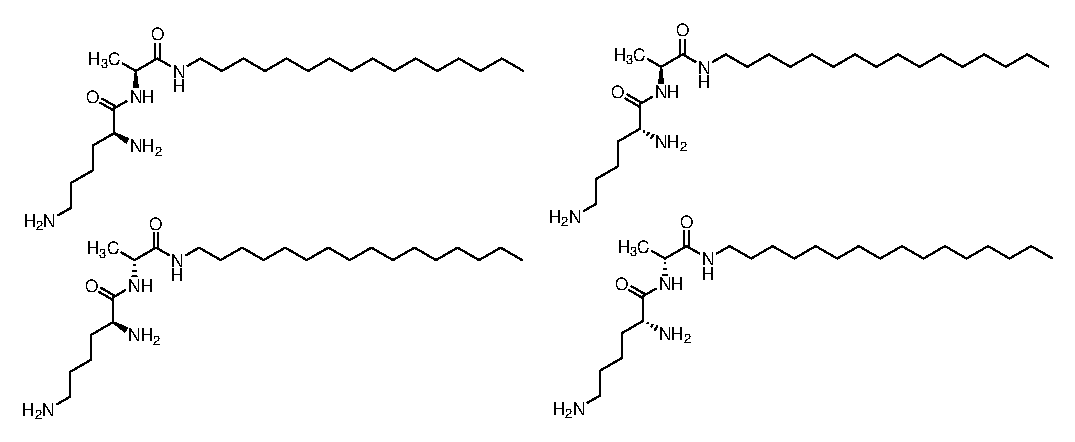
\includegraphics[scale=0.9]{Figures/C16-Ala-Lys_family.eps}
\caption{ The novel self-assembling heparin binders synthesised in this work. \newline
L-R Top row: C\textsubscript{16}-L-Ala-L-Lys, C\textsubscript{16}-L-Ala-D-Lys. Bottom row: C\textsubscript{16}-D-Lys-L-Ala, C\textsubscript{16}-D-Ala-D-Lys}
\label{C16-Ala-Lys_family}
\end{figure}

The use of the alanine spacer here is an extension of previous work by Chan \textit{et al.}\textsuperscript{\cite{Chan2016ChiralBinding}} The original work used a glycine amino acid as a spacer group between the C\textsubscript{16} carbon chain and the lysine binding group. It was this spacer group which appeared to give this self-assembled interface chiral selectivity towards DNA, with the effect being less pronounced on binding to heparin sulfate. It was hypothesised by the researchers that the difference in chiral selectivity is perhaps due to the more polydisperse nature of heparin. Glycine is unique in the sense it is the only achiral naturally occurring amino acid. By changing the glycine spacer to an alanine residue, we hoped to elucidate whether the chirality of the spacer group also has any effect on the binding to heparin and/or DNA. 

The inclusion of the carbon chain as a hydrophobic group drives the self assembly of these nanoscale compounds, due to the hydrophobic effect.\textsuperscript{\cite{Rodrigo2011Self-AssemblingBinding}} It is known from previous work by Vieira, Albanyan \textit{et al.} that there is a fine balance between the size of the hydrophobic and hydrophilic components of the molecule.\textsuperscript{\cite{Vieira2017EmergenceHeparin}}
If the balance is tipped too far in either direction, the molecule either does not self-assemble as the hydrophobic carbon chain is not large enough to drive the self-assembly, or the nanoscale interface is poorly soluble in aqueous media and hence unsuitable for its desired purpose. For this reason, a C\textsubscript{16} carbon chain was chosen as the hydrophobic component for this family of nanoscale heparin binders, as we reason it is sufficiently hydrophobic to drive self-assembly, without adversely affecting the molecule's solubility in aqueous media. 
\newpage
\section{Project Aims}
As a result of the issues outlined above, it would be clinically useful if we could develop systems to do two things: 
\begin{enumerate}
\item to develop another rescue agent with a favourable toxicological and pharmacokinetic profile to replace protamine sulfate, or to develop a rescue agent which binds only to the active parts of heparin. 
\item to develop a non-viral vector agent which binds DNA, and possesses a greater potency than those already in existence. 
\end{enumerate}
The work herein attempts to approach these issues and synthesise a potential protamine sulfate mimic, or a new non-viral vector suitable for gene therapy.

In order to achieve this however, it is necessary to understand in more detail the binding interface between heparin sulfate and synthetic nanoscale systems. In particular, we are interested in the importance of chirality in mediating specific binding between heparin sulfate or DNA and these synthetic systems. With this in mind, the aims of this project are therefore as follows:
\begin{itemize}
\item To synthesise a family of related palmitic acid based molecules, with a variety of chiralities - two pairs of enantiomers which have a diastereomeric relationship with each other (Figure \ref{C16-Ala-Lys_family}). 
\item To characterise these molecules using \textsuperscript{13}C,\textsuperscript{1}H NMR and DEPT-135, alongside Mass Spectrometry and Infrared Spectroscopy to prove the expected compounds have been synthesised. 
\item To assess the degree of self-assembly of these molecules using TEM, DLS and Nile Red competition assays.
\item To assess the DNA binding ability of these novel molecules using Ethidium Bromide competition assays. 
\item To assess the heparin binding ability of these potential protamine sulfate mimics using a Mallard Blue assay. 
\end{itemize} 

We hope to explore whether the enantiomeric selectivity between heparin and DNA demonstrated previously by Chan and Bromfield is a general outcome of inserting any amino acid between the C\textsubscript{16} carbon chain and the lysine binding group.\textsuperscript{\cite{Bromfield2015HeparinNanostructures,Chan2016ChiralBinding}} If this is the case, we can then tune the binding of the lysine group to preferentially bind the biological polyanions of our choosing. This would demonstrate that the design of synthetic systems with greater selectivity, and potentially fewer side effects than protamine sulfate is possible. 
